\section{目的}

依講義 PDF 第 65--73 頁，重建 MOS/TG 充放電、六種傳輸鏈、直流電流路徑、浮接保持與傳輸閘全加器。比較的核心是通道截止造成的電位損失、串接 RC、回復器的負載代價與動態節點保持時間。

\section{講義要求與對應測試}

\begin{center}
\small
\setlength{\tabcolsep}{4pt}
\begin{tabular}{p{.42\linewidth}p{.29\linewidth}p{.18\linewidth}}
\toprule
要求 & 網表編號與條件 & 狀態 \\
\midrule
步驟 1：表 16.1/16.2 六種充放電 & 01; 20 fF, 10 ns & 已量測 \\
步驟 2：六種四開關鏈與中間反相器 & 02; 0.2 ns edges & 雙方向已量測 \\
問題 1：電流隨輸出電位的路徑 & 03; DC 0--1 V & 已量測 \\
問題 2：微秒尺度 TG 保持 & 04; 25/115 C, 20 us & 已量測 \\
問題 3：全加器與兩輸出延遲 & 05; 8 vectors, 5 fF & 8/8；延遲已量測 \\
\bottomrule
\end{tabular}
\end{center}

\section{電路與推導}

NMOS 傳高時 $V_{GS}$ 隨輸出上升而減少，近似截止於 $V_o\simeq V_{DD}-V_T(V_{SB})$；PMOS 傳低則保留約 $|V_{TP}|$ 的殘餘電壓。Body effect 使門檻隨節點電位改變，因此不能直接用常數 $V_T$ 把曲線當直線。TG 的 N/P 並聯互補傳高與傳低能力。

鏈 1/2 使用 PMOS，3/4 使用 NMOS，5/6 使用 TG；偶數鏈在第 2 與第 3 開關之間加入反相器，故輸入到輸出極性與奇數鏈相反。鏈 6 前兩個 PMOS 的 $L=0.6\,\mu$m 按表 16.3 掃描頁可見數值實作，其餘如網表所列；此不對稱與掃描歧義保留，不擅自全部改為 $0.25\,\mu$m。

全加器用 TG 多工器表示圖 16.3 的邏輯，令 $P=A\oplus B$，則 $S=P\oplus C$、$C_{out}=\overline P B+PC$。Sum 與 Carry 各有一級輸出反相器；補數資料在 TG 前產生，以免把最後反相器的反相作用漏算。這是明列的邏輯等價 TG 實作，不把其延遲宣稱為掃描圖內部寄生的精確重現。

\section{模擬設定與判讀方式}

以提供的加密 MOS 模型、1.0 V 供應、25\,$^\circ$C 為基準。1.0 V 是教學測試條件，並非已核實的額定電壓；沒有把本次結果當作講義原製程或原供應電壓的重現。除網表另註，$W_n/W_p/L=0.6/1.8/0.25\,\mu\mathrm m$，Bulk 接對應電源軌，輸出負載為 5 fF。傳輸閘與弱回授器件的例外尺寸均在網表明列。

使用 PrimeSim HSPICE S-2021.09 win64、\texttt{RUNLVL=6}、\texttt{ACCURATE} 及 \texttt{WARNLIMIT=100}。每份網表的主分析與 \texttt{.alter} 均完成，沒有 error 或 failed measurement；但模擬器仍回報加密區塊的警告被隱藏，因此不能宣稱模型無警告或警告無害。\texttt{.tran} 的列印間隔不是固定積分步長；求解器使用自適應步長。本次沒有把有限的掃描範圍當作完整製程認證。

除非另註，功能診斷以低電位 $V\leq0.2$ V、高電位 $V\geq0.8$ V 判定；這是本報告公開採用的判讀規則，不是講義給定的數值門檻，也不是已萃取的接收器雜訊容限。取樣正確不能排除取樣間毛刺。所有圖均由實際輸出資料重繪；\texttt{results/} 保存逐案例波形、量測與衍生比較 CSV。

公開網表不含模型載入路徑；模擬時在本機副本加入模型設定，模型本體不在交付資料內。網表檔名的前兩位數對應下表編號，各檔可獨立執行。

\section{結果}

\subsection{端點電位與鏈延遲}

\begin{center}
\small
\setlength{\tabcolsep}{4pt}
\begin{tabular}{lr}
\toprule
路徑 & 10 ns 電位 (V) \\
\midrule
PMOS charge & 1.000001 \\
PMOS discharge & 0.347873 \\
NMOS charge & 0.642986 \\
NMOS discharge & 0.000004 \\
TG charge & 1.000003 \\
TG discharge & 0.000004 \\
\bottomrule
\end{tabular}
\end{center}

\begin{figure}[htbp]
\centering
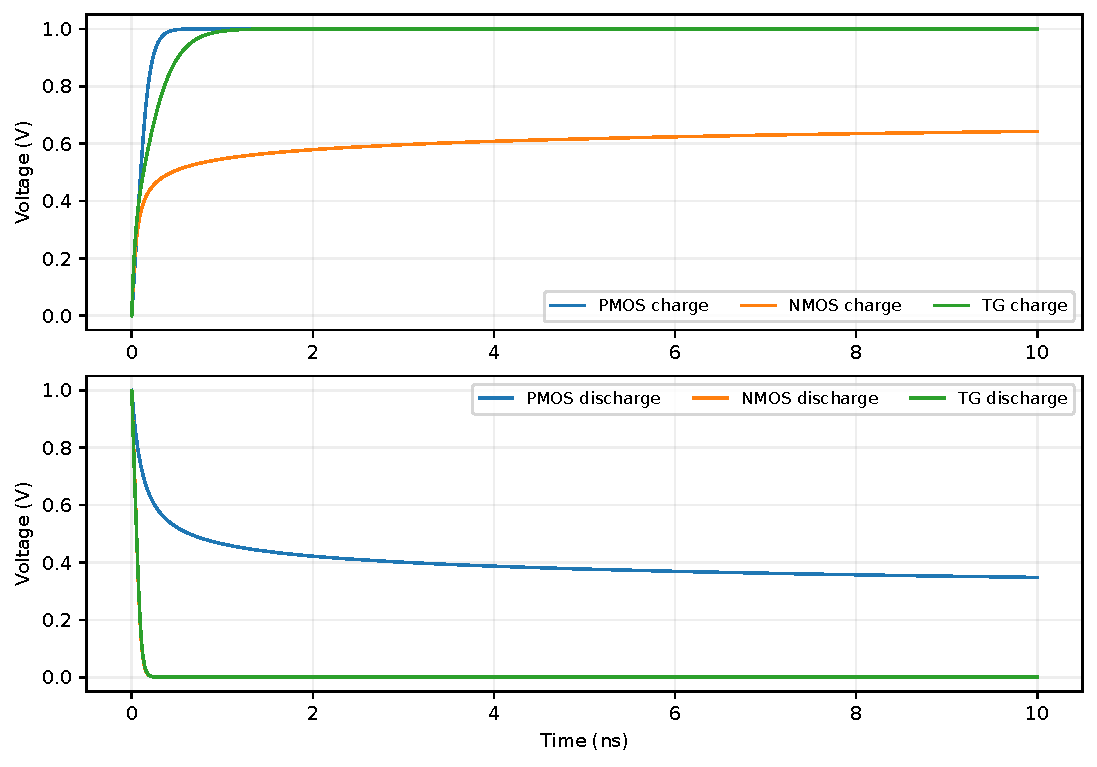
\includegraphics[width=.96\linewidth]{figures/pass_device_levels.pdf}
\caption{六種初始電容充放電；單一 MOS 的弱傳輸方向未達完整電源軌。}
\end{figure}

\begin{center}
\small
\setlength{\tabcolsep}{4pt}
\begin{tabular}{lrr}
\toprule
鏈 & 輸入上升延遲 (ns) & 輸入下降延遲 (ns) \\
\midrule
1 & 5.2722 & 0.6198 \\
2 & 3.1878 & 2.3384 \\
3 & 0.2843 & 1.9191 \\
4 & 1.1735 & 1.4468 \\
5 & 0.4430 & 0.9402 \\
6 & 0.7254 & 1.1440 \\
\bottomrule
\end{tabular}
\end{center}

延遲是輸入與對應輸出 50\% 交點之差，偶數鏈依反相極性選取輸出方向。PMOS 鏈 1 的上升延遲 5.2722 ns 對中點回復後的鏈 2 為 3.1878 ns；但鏈 2 的另一方向反而變慢。因此中間反相器不是每一方向都必然加速。

\begin{figure}[htbp]
\centering
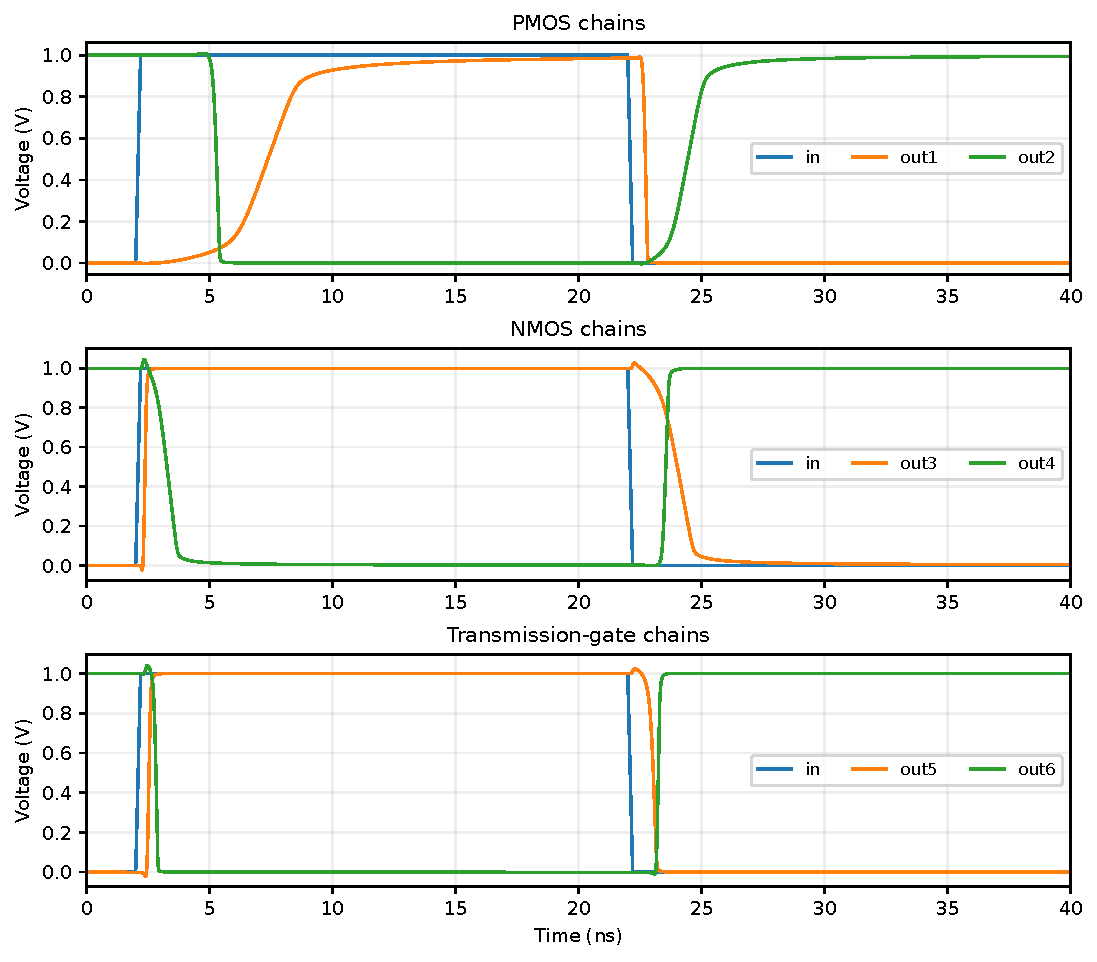
\includegraphics[width=.96\linewidth]{figures/six_chains.pdf}
\caption{六鏈完整輸入與輸出波形；含中間反相器的鏈輸出極性不同。}
\end{figure}

\subsection{直流電流與動態保持}

\begin{figure}[htbp]
\centering
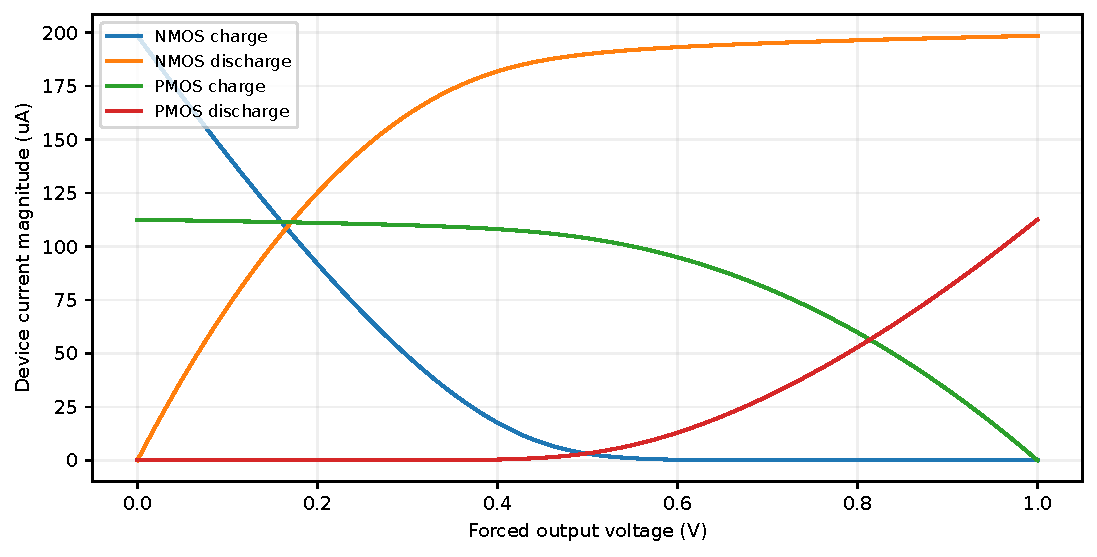
\includegraphics[width=.96\linewidth]{figures/current_trajectories.pdf}
\caption{把輸出強制掃描 0--1 V，呈現四個單 MOS 的充放電電流路徑。}
\end{figure}

例如輸出 0.5 V 時，NMOS 充電/放電電流為 3.0819/189.9322\,$\mu$A，PMOS 為 103.8178/3.2356\,$\mu$A，直接解釋兩者相反的弱傳輸方向。浮接節點滿足 $C\,dV/dt=-I_{\rm net}(V,T)$；保持時間需要按實際可接受電位定義。

\begin{center}
\small
\setlength{\tabcolsep}{4pt}
\begin{tabular}{lrrrr}
\toprule
溫度 (C) & 初始 (V) & 5 us (V) & 20 us (V) & 至 0.8 V (us) \\
\midrule
25 & 1.0372 & 0.8926 & 0.6496 & 9.868 \\
115 & 1.0385 & 0.5252 & 0.0001 & 2.076 \\
\bottomrule
\end{tabular}
\end{center}

\begin{figure}[htbp]
\centering
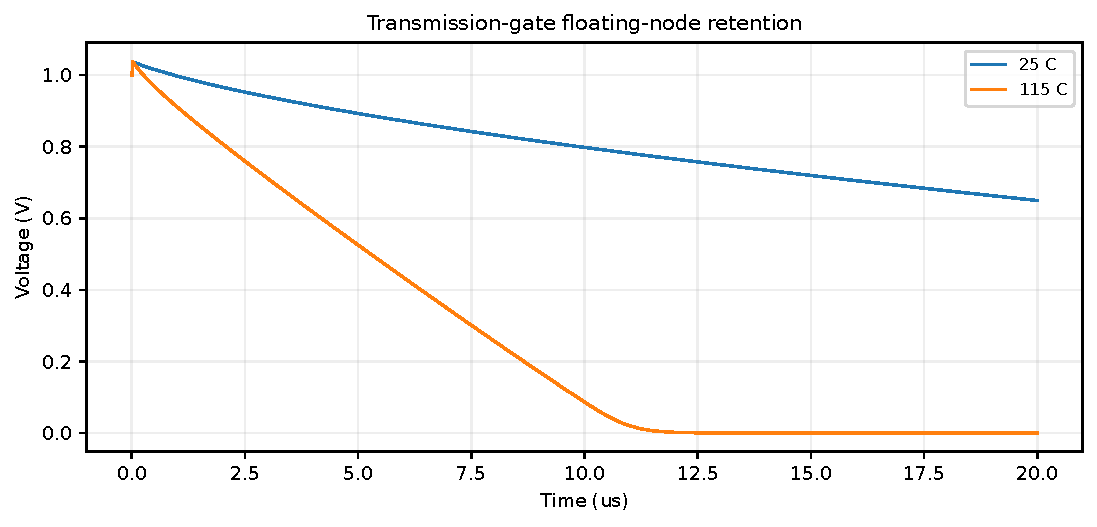
\includegraphics[width=.96\linewidth]{figures/retention.pdf}
\caption{TG 關閉後的 20 fF 節點保持；起始略高於 1 V 是時脈耦合。}
\end{figure}

若系統浮接時間為半個週期，可用表中 $t_{0.8}$ 估算 $f\gtrsim1/(2t_{0.8})$；實際刷新還須保留餘量，且取決於讀取門檻、負載及溫度。這不是由單次測試得到通用最小時脈頻率。

\subsection{全加器}

\begin{center}
\small
\setlength{\tabcolsep}{4pt}
\begin{tabular}{lrrr}
\toprule
ABC & 預期 S/C & Sum (V) & Carry (V) \\
\midrule
000 & 0/0 & 0.00000 & 0.00000 \\
001 & 1/0 & 1.00000 & 0.00000 \\
010 & 1/0 & 1.00000 & 0.00000 \\
011 & 0/1 & 0.00000 & 1.00000 \\
100 & 1/0 & 1.00000 & 0.00000 \\
101 & 0/1 & 0.00000 & 1.00000 \\
110 & 0/1 & 0.00000 & 1.00000 \\
111 & 1/1 & 1.00000 & 1.00000 \\
\bottomrule
\end{tabular}
\end{center}

8 種輸入均得到正確穩態邏輯。選取 A=0、B=1、Cin 在 30 ns 上升的單一敏化轉換，Sum 下降延遲為 171.814 ps，Carry 上升為 177.449 ps；這是指定向量下的兩條路徑，並非全向量最壞延遲。

\begin{figure}[htbp]
\centering
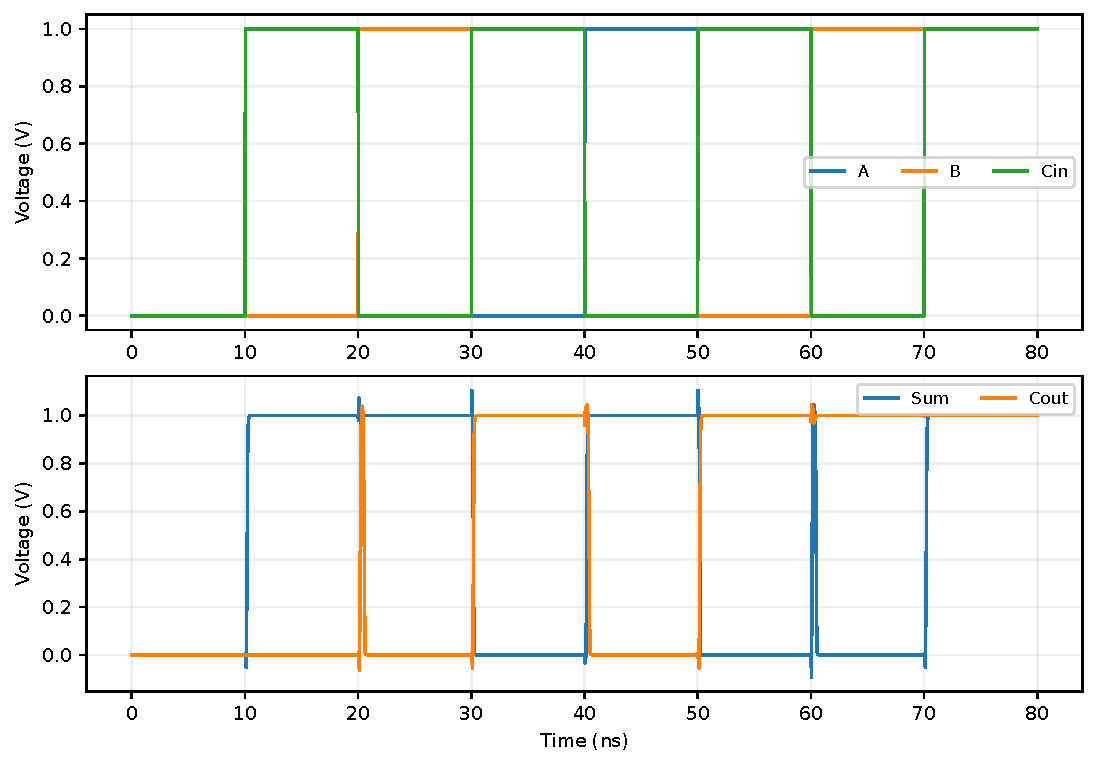
\includegraphics[width=.96\linewidth]{figures/adder.pdf}
\caption{全加器 8 個輸入向量與 Sum/Carry 輸出。}
\end{figure}

\section{討論、差異與尚未證實的範圍}

原資料作為參考，實作按講義逐項建立獨立 testbench，補足直流路徑、保持時間與完整真值表。充放電初始條件、負載和串接極性均顯式列出。單 MOS 的有限時間端點不能直接當作精確門檻萃取；TG 仍有有限電阻、寄生耦合及漏電。CSV 可用於重算門檻及延遲。
